\documentclass{ximera}

\title{Oefening op de methode der halfwaardetijden}
\author{Mila Vervoort}
\license{CC: 0}         % replace with an appropriate license, or set it in xmPreamble

\begin{document}
\begin{abstract}
    Oefening op de methode der halfwaardetijd
\end{abstract}
\maketitle
\label{xim:Oefening methode der halfwaardetijden}

\section*{Oefening 1: Langmuir-Hinshelwood kinetica}

\textbf{Gegeven}

Beschouw de reactiekinetica:
\[
-R_A = \frac{k_1 C_A}{1 + k_2 C_A}
\]

Er werden kinetische experimenten gedaan in een batchreactor. Voor verschillende beginconcentraties werd de halfwaardetijd gemeten:

\[
\begin{array}{c|c}
C_{A0} \ (\text{mol/L}) & t_{1/2} \ (\text{s}) \\
\hline
0.5 & 1.7 \\
1.0 & 2.4 \\
1.5 & 3.1 \\
2.0 & 3.8 \\
2.5 & 4.5 \\
\end{array}
\]

\textbf{Gevraagd}

Bepaal de waarden van $k_1$ en $k_2$.


\begin{question} \textbf{Uitdrukking voor de halfwaardetijd zoeken}

\begin{multipleChoice}
\choice{$t_{1/2} = \frac{\ln(2)}{k_1} + \frac{k_2 C_{A0}}{k_1}$}
\choice[correct]{$t_{1/2} = \frac{\ln(2)}{k_1} + \frac{k_2 C_{A0}}{2k_1}$}
\choice{$t_{1/2} = \frac{\ln(2)}{k_1} - \frac{k_2 C_{A0}}{2k_1}$}
\choice{$t_{1/2} = \frac{1}{k_1} \ln(2 + k_2 C_{A0})$}
\end{multipleChoice}

\begin{feedback} \text{  }

Vertrek van de geïntegreerde vorm:
\[
\ln\left(\frac{C_{A0}}{C_A}\right) + k_2 (C_{A0} - C_A) = k_1 t
\]
Voor de halfwaardetijd geldt $C_A = C_{A0}/2$. Invullen geeft:
\[
\ln(2) + k_2 \left(C_{A0} - \frac{C_{A0}}{2}\right)
= k_1t_{1/2}
\]
Dus:
\[
t_{1/2} = \frac{\ln(2)}{k_1} + \frac{k_2 C_{A0}}{2k_1}
\]
Herschrijf als een rechte:
\[
\underbrace{t_{1/2}}_{y}
=
\underbrace{\frac{\ln(2)}{k_1}}_{\text{intercept } b}
+
\underbrace{\frac{k_2}{2k_1}}_{\text{helling } m}
\cdot
\underbrace{C_{A0}}_{x}
\]
\end{feedback}
\end{question}

\begin{question} \textbf{Interpreteren van de plot}

De data wordt uitgezet in een $t_{1/2}$ vs $C_{A0}$ grafiek.

\begin{center}
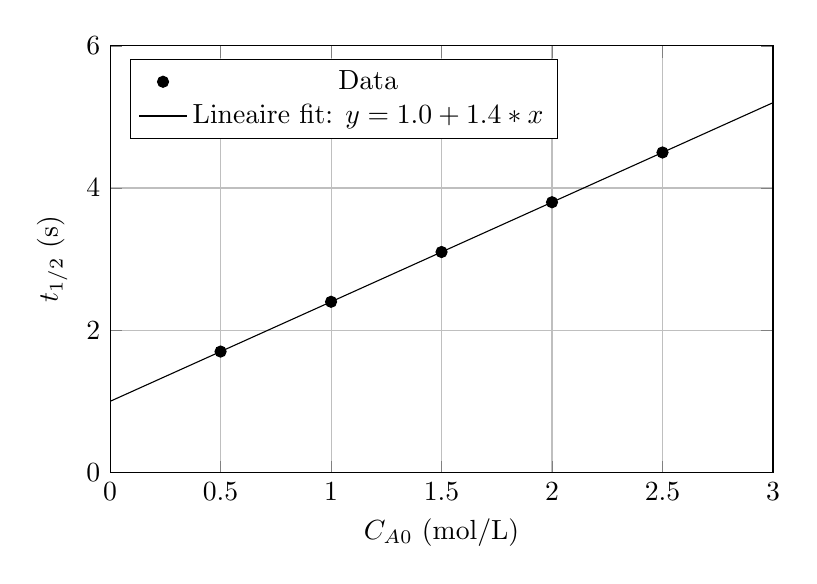
\begin{tikzpicture}
\begin{axis}[
    xlabel={$C_{A0}$ (mol/L)},
    ylabel={$t_{1/2}$ (s)},
    grid=major,
    width=10cm,
    height=7cm,
    xmin=0, xmax=3,
    ymin=0, ymax=6,
    legend pos=north west,
]

% Data punten
\addplot[
    only marks,
    mark=*,
] coordinates {
    (0.5,1.7)
    (1.0,2.4)
    (1.5,3.1)
    (2.0,3.8)
    (2.5,4.5)
};

% Regressielijn
\addplot[
    domain=0:3,
    samples=100,
] {1.0 + 1.4*x};

\legend{Data, Lineaire fit: $y = 1.0 + 1.4*x$}

\end{axis}
\end{tikzpicture}
\end{center}

Hieruit kan worden afgeleid dat:
\[k_1 = \answer{0.69} \text{ s}^{-1}\]
\[k_2 = \answer{1.94} \text{ L/mol}\]

\begin{feedback} \text{  }

    Het intercept: $\frac{\ln(2)}{k_1}$ = 1.0
    \[k_1 = \frac{\ln(2)}{1.0} \text{ s}^{-1}\]
    De helling: $\frac{k_2 C_{A0}}{2k_1} = 1.4$
    \[k_2 = 2 k_1 \cdot 1.4 = 1.94 \text{ L/mol} \]
\end{feedback}
\end{question}

\end{document}